\chapter{Static Scheduling}

Dynamic scheduling (out of order scheduling) requires significant hardware complexity.
\begin{itemize}
    \item Register Update Units, reorder buffers, registers backed by commit registers and associated with tags, instruction dependency checks.
    \item All of these take space on the die (not only does a larger chip necessitate fewer chips per wafer, but the yield is also decreased)
    \item Also requires more energy, results in more heat and hence lower thermal limits.
    \item The complexity of determining the number of instructions that can safely be issued in parallel is $O(n^2)$, which is achievable for small $n$, but can necessitate more stages between fetch and issue.
\end{itemize}
With static scheduling this complexity is removed from hardware, and moved to the compiler, with the ISA providing necessary mechanisms to express how instructions should be scheduled (e.g in parallel).

\section{Software Pipelining}
\begin{center}
    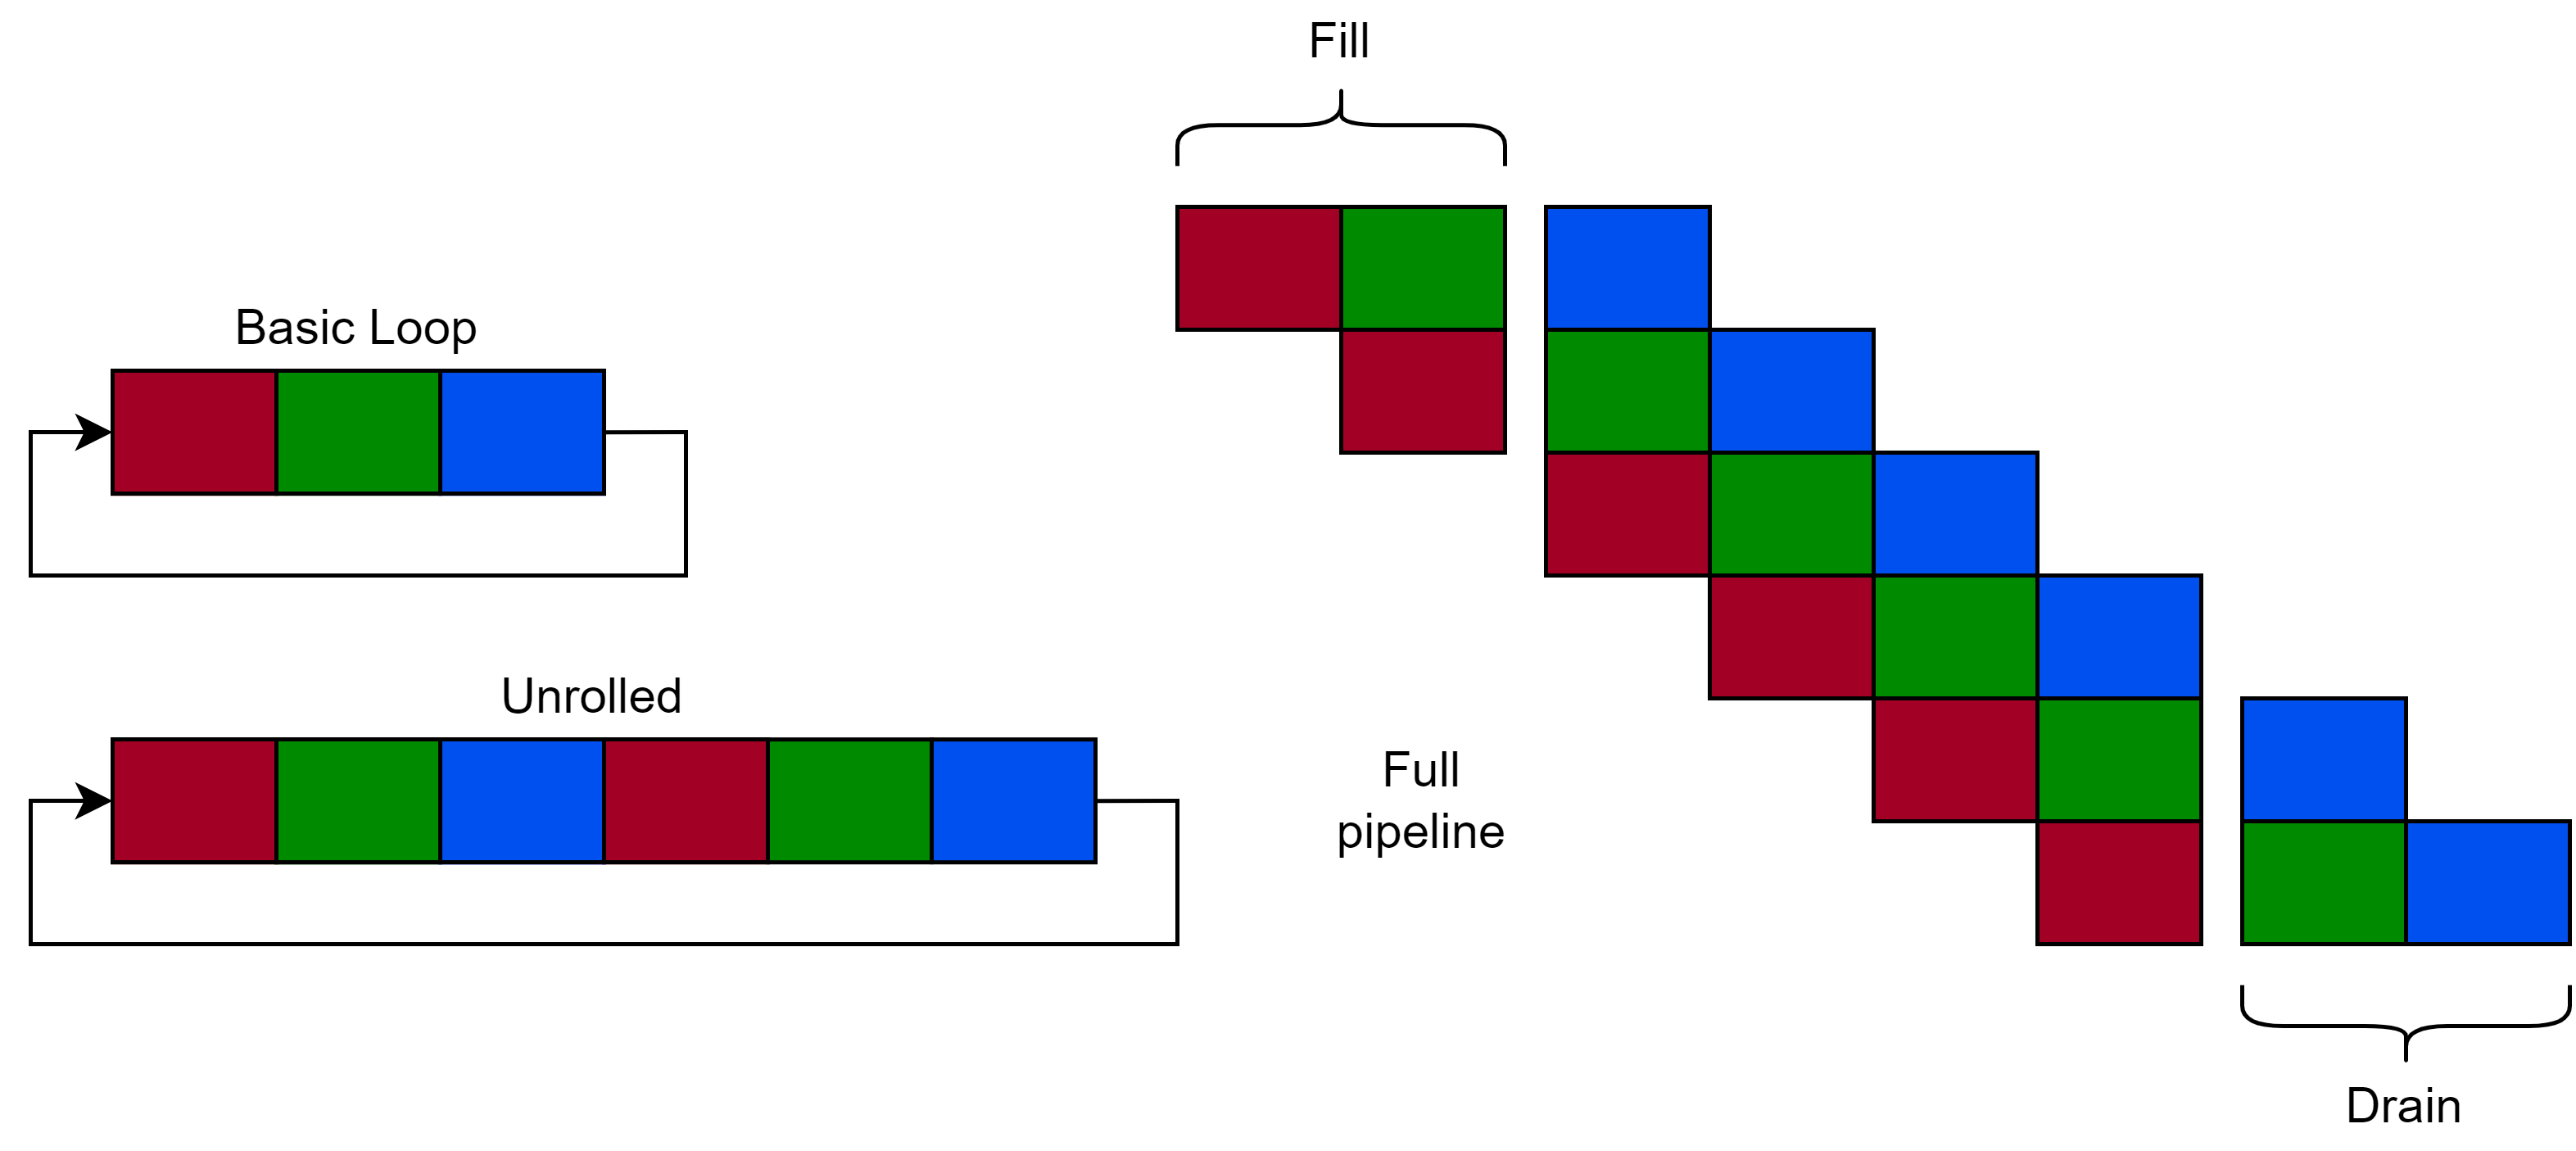
\includegraphics[width=\textwidth]{static_scheduling/images/software_pipelining.drawio.png}
\end{center}

We can pipeline loop iterations, in the diagram above the basic loop and unrolled loop both execute the loop contents in order. By pipelining each of the 3 instructions in the loop body are run for 3 different in-order \textit{iterations}.
\begin{itemize}
    \item e.g iteration $3$ is in red, while $2$ is in green and $1$ is in blue.
    \item Increases the load-use distance, so removes/reduces stall potential.
\end{itemize}

\section{Very Lond Instruction Word}
\begin{definitionbox}{Very Lond Instruction Word (VLIW)}
    Each instruction contains encodings for multiple operations.
    \begin{itemize}
        \item All operations are independent and hence can be issued and executed in parallel.
        \item The compiler/programmer needs to extract dependencies, and work out which instructions can be issued \& executed in parallel, rather than the hardware.
        \item Instructions become large, and where there is little parallelism to be extracted, majority of the instructions are mostly no-ops.
        \item Large instructions put pressure on memory access bandwidth.
        \item Often not binary compatible across generations (e.g number of functional units change, instruction size changes)
    \end{itemize}
\end{definitionbox}
With software pipelining we can schedule instructions for different stages of the pipeline in parallel.

\section{Explicitly Parallel Instruction Computing}
\begin{definitionbox}{Explicitly Parallel Instruction Computing (EPIC)}
    A term created by Intel \& HP, considered to be the next generation of VLIW. 
    \begin{itemize}
        \item Often used to refer to IA-64 (Itanium) processors.
        \item ISA exposes parallelism to the compiler.
        \item Binary compatible across generations/processor implementations.
    \end{itemize}
\end{definitionbox}

In IA-64 instructions are encoded in bundles, each 128 bits wide:
\begin{itemize}
    \item $5$ bit template field encodes which instructions can be run in parallel in the bundle (where the $;;$ / $stop!$ is, after which the next set of parallel instructions begin)
    \item $3$ instructions, each with $41$ bits of length, this allows for large number of registers, large immediate operands.
\end{itemize}
Itanium also included a large number of features to expose 